\section{Initialization\label{sec:experimental_procedure}}
To generate silica in the glass form we first create a perfect silica crystal in the crystalline form $\upbeta$-cristobalite, the unit cell of which can be seen in figure \cref{fig:beta_cristobalite-unit_cell}, and a larger crystal in \cref{fig:cristobalite_crystal}. This crystalline form consists of corner-bonded SiO$_4$-tetrahedra, and in the perfect crystallic form all silicon atoms are bound to four oxygen atoms, and all oxygen atoms to two silicon atoms. 

We give the atoms a random uniformly distributed velocities with mean $\mu = 0$ and standard deviation $\sigma \propto \sqrt{T}$, where $T$ is the wanted temperature.%
\begin{figure}[htb]%
    \centering%
    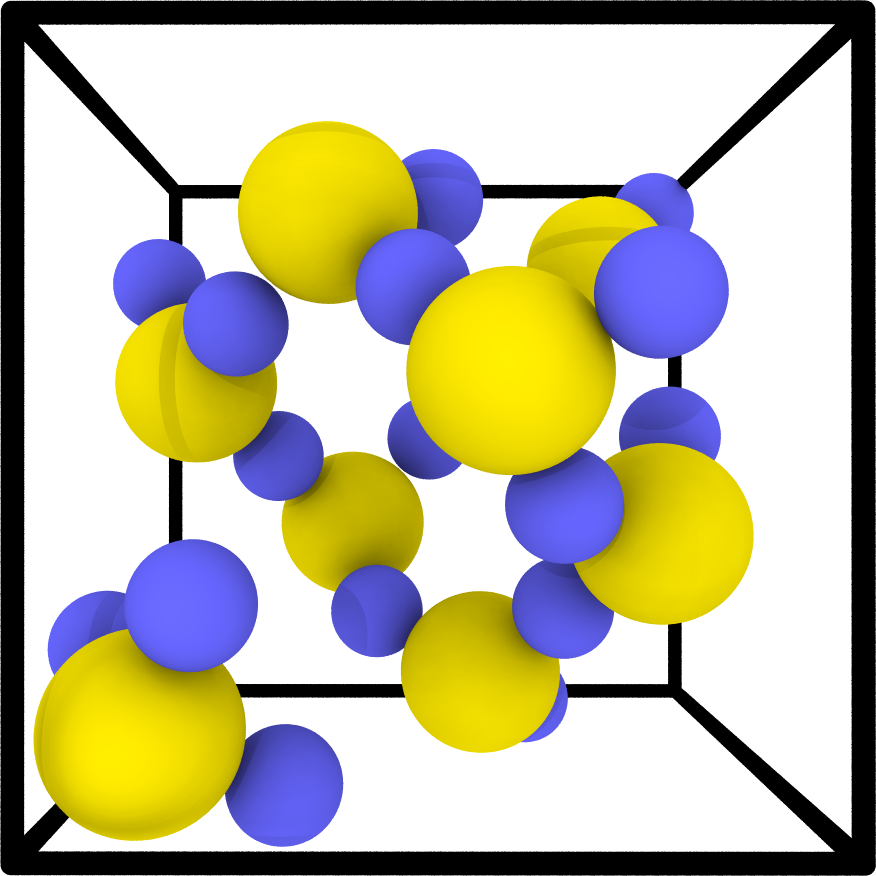
\includegraphics[width=0.4\textwidth]{images/beta_cristobalite/unit_cell05_cropped.png}%
    \caption{%
        $\upbeta$-cristobalite unit cell, with 8 silicon atoms and 16 oxygen atoms.%
        \label{fig:beta_cristobalite-unit_cell}%
    }%
\end{figure}%

We then heat the system to 4500 K in steps of 700 K to melt the silica crystal. Since we are mainly interested in controlling the temperature at this stage, the Berendsen thermostat is used for these temperature changes. We alternate between using a thermostat to adjust the temperature, and simulating with the thermostat off, to let the system thermalize and react to the temperature change after applying the thermostat. The number of timesteps we used for the thermostat period is around 2 500, and for the thermalization period around 10 000. We then cool the system by doing the previous procedure in reverse. See \cref{fig:plot_heat_melt_sio2} for a plot of the temperature as function of time while we melt and cool down the system, and \cref{fig:initialization_step00} for a visualization of a perfect crystal of $\upbeta$-cristobalite, and \cref{fig:initialization_step02} for amorphous, solid silica.%
%
\begin{figure}[htpb]%
    \centering%
    \includesvg[width=0.6\textwidth, svgpath = ./images/energy_plots/]{system00_temperature_melt_cool}%
    \caption{%
        Plot of the temperature (in kilo-Kelvin) as function of timesteps when melting and cooling down a silica system, using the Berendsen thermostat. We use timesteps of 0.050 picoseconds, and use 2 500 timesteps with the thermostat turned on, and then 10 000 timesteps to let the system thermalize (with the thermostat off), for each step in temperature. %
        \label{fig:plot_heat_melt_sio2}%
    }%
\end{figure}%
%
% \todob{Reference figures below, say something about energy conservation \cref{fig:plot_heat_melt_sio2,fig:plot_energy_conservation}}
% \todoco{Silica phase diagram? for melting, phases etc. - Not needed according to Malthe}

The initialization procedure is visualized in \cref{fig:initialization_steps}, and can be summed up as follows
\begin{itemize}
    \item Generate a perfect crystal of $\beta$-cristobalite of the wanted size (\cref{fig:initialization_step00}).
    \item Heat the system to well above the melting point of silica (we usually use 4 500 Kelvin, using a thermostat (Berendsen) (\cref{fig:initialization_step01}).
    \item Cool down the system to well below the glass-transition temperature (we use 300 Kelvin), using a thermostat (Berendsen) (\cref{fig:initialization_step02}).
    \item Cut out the fracture (\cref{fig:initialization_step03}).
    \item Passivate the dangling ends and apply steepest descent to let the passivation atoms find their optimal positions (\cref{fig:initialization_step04}).
    \item Fill the pore with water, and thermalize the system at 300 K (\cref{fig:initialization_step05}).
\end{itemize}
%
\begin{figure}[htpb]%
%     \captionsetup{width=1.4\textwidth}%
    \setlength{\myfigwidth}{0.35\textwidth}%
    %
    \setlength{\myhfillwidth}{1.5cm}%
    \centering%
    \begin{subfigure}[t]{\myfigwidth}
        \captionsetup{width=1.1\textwidth}%
        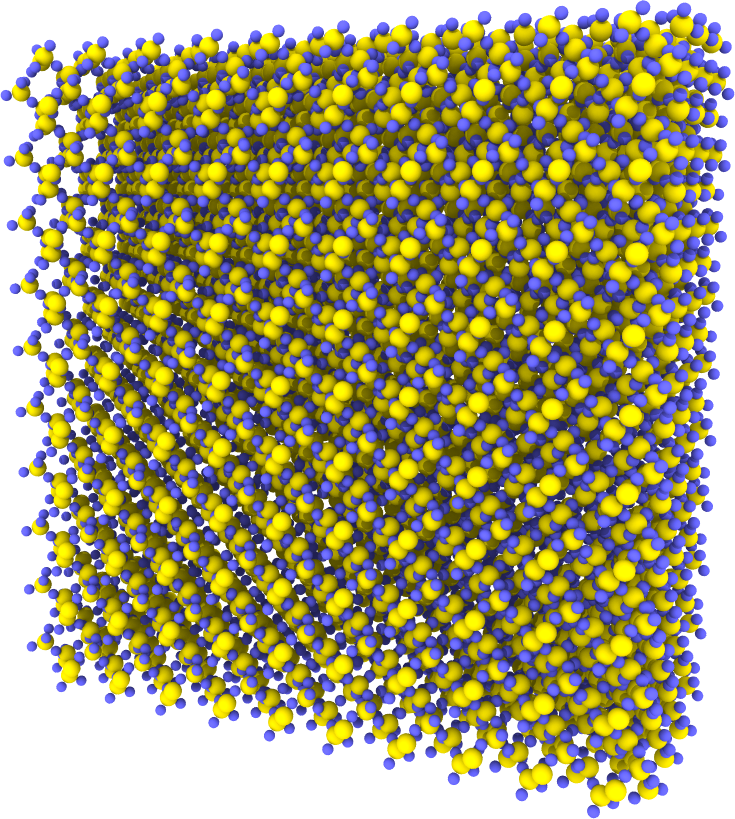
\includegraphics[width=\textwidth]{images/experimental_procedure/00_10}%
        \caption{%
            Perfect $\upbeta$-cristobalite crystal.%
            \label{fig:initialization_step00}%
            \label{fig:cristobalite_crystal}%
        }%
        \hspace{8pt}
    \end{subfigure}%
    \hspace{\myhfillwidth}%
    \begin{subfigure}[t]{\myfigwidth}%
        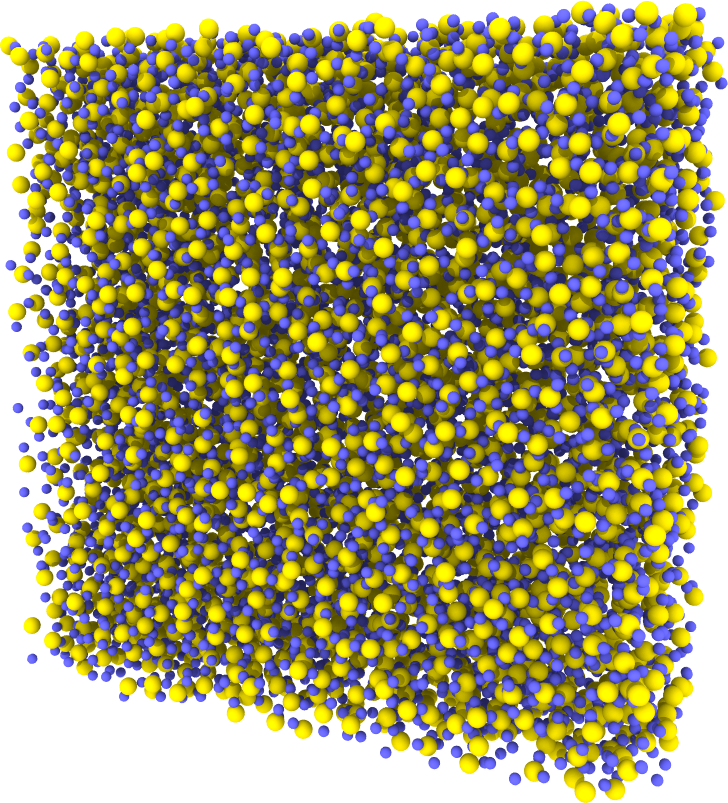
\includegraphics[width=\textwidth]{images/experimental_procedure/01_10}%
        \caption{%
            Silica heated to 4500 K.%
            \label{fig:initialization_step01}%
        }%
        \hspace{8pt}
    \end{subfigure}%
    \\%
    \begin{subfigure}[t]{\myfigwidth}%
        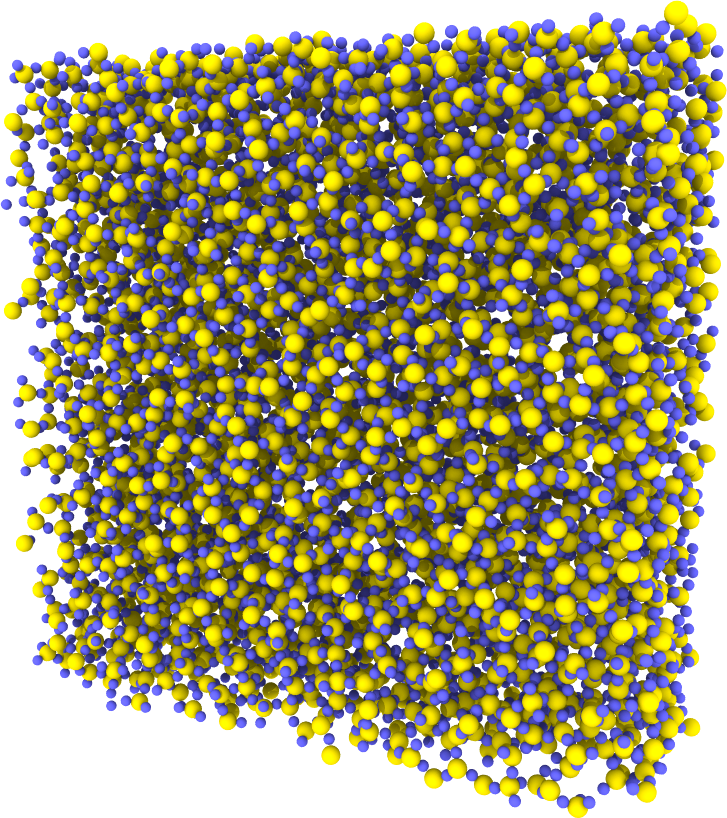
\includegraphics[width=\textwidth]{images/experimental_procedure/02_10}%
        \caption{%
            Silica cooled to 300 K.%
            \label{fig:initialization_step02}%
        }%
    \end{subfigure}%
    \hspace{\myhfillwidth}%
    \begin{subfigure}[t]{\myfigwidth}%
        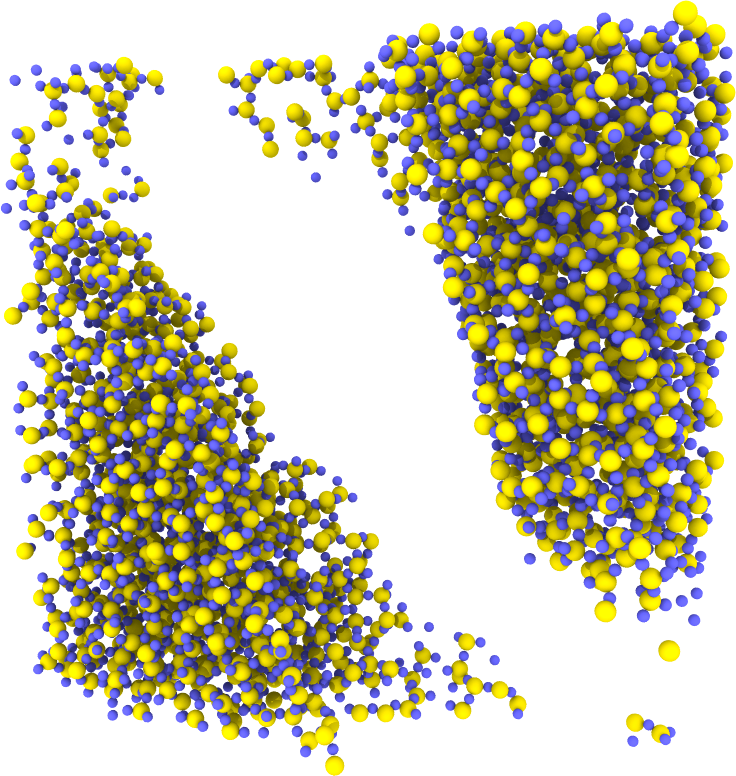
\includegraphics[width=\textwidth]{images/experimental_procedure/03_10}%
        \caption{%
            Fracture cut out.%
            \label{fig:initialization_step03}%
        }%
        \hspace{8pt}
    \end{subfigure}%
    \\%
    \begin{subfigure}[t]{\myfigwidth}%
        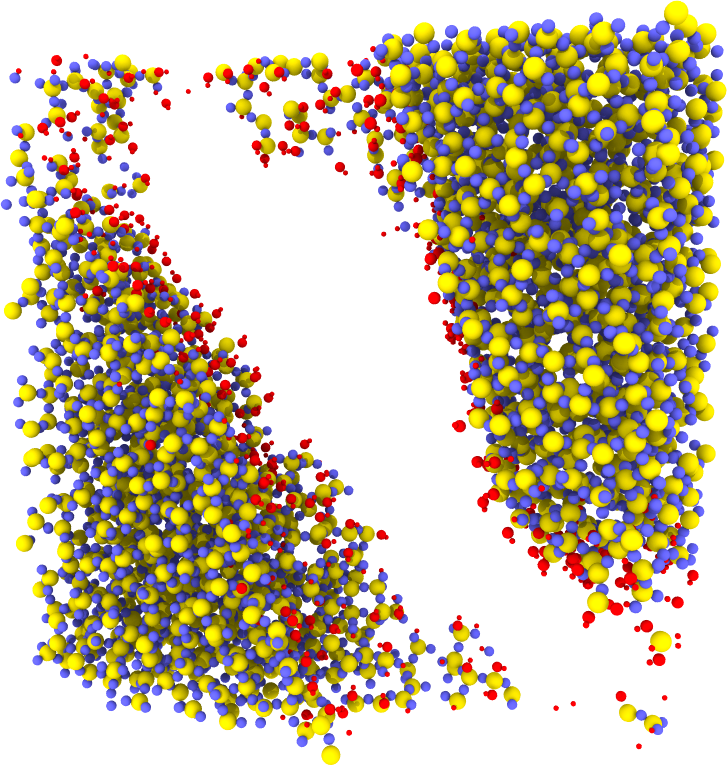
\includegraphics[width=\textwidth]{images/experimental_procedure/04_10}%
        \caption{%
            Dangling ends passivated.%
            \label{fig:initialization_step04}%
        }%
        \hspace{8pt}
    \end{subfigure}%
    \hspace{\myhfillwidth}%
    \begin{subfigure}[t]{\myfigwidth}%
        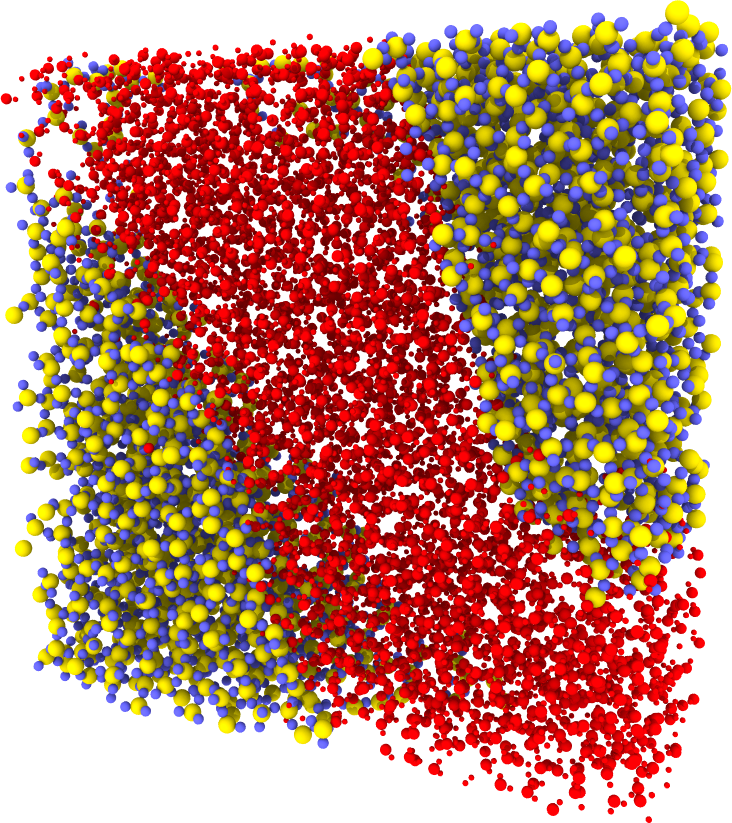
\includegraphics[width=\textwidth]{images/experimental_procedure/05_10}%
        \caption{%
            Pore filled with water.%
            \label{fig:initialization_step05}%
        }%
        \hspace{8pt}
    \end{subfigure}%
    \captionsetup{width=\textwidth}%
    \caption{%
        Visualizations of the different stages of initialization of a fracture in silica filled with water. We show a $75\times 75\times 25$ \AA\ slice of a much larger system $(172 \text{ \AA})^3$. The silicon atoms are yellow, the silica-oxygen blue, and hydrogen and water-oxygen red. %
        \label{fig:initialization_steps}%
    }%
\end{figure}%

We now have a thermalized and (hopefully) realistic silica crystal at near room temperature. From this crystal we cut out the fracture, passivate using one of the passivation methods, and fill the fracture with water molecules, \hl{and use steepest descent}. After filling the fracture with water we need to thermalize the system again, since the energy (and thereby the temperature) changes when we remove and insert atoms.